\documentclass[12pt]{article}
\usepackage[utf8]{inputenc}
\usepackage{graphicx}
%\usepackage[margin=0.5in]{geometry}
\usepackage{hyperref}
\title{\Huge{Unbabel Java Challenge}}
\author{Tomasz Szypuła}
\date{\today}

\begin{document}
\maketitle
\section{Project Overview and Objectives }
\paragraph{The goal}of the challenge was to write a Java Application meeting the requirements specified in the \href{ https://github.com/Unbabel/java-coding-challenge}{java-coding-challenge}. The main resources I have chosen to use in this task are 
\begin{itemize}
\item \href{https://docs.oracle.com/javase/8/javafx/get-started-tutorial/jfx-overview.htm#JFXST784}{JavaFX GUI framework} which provides tools for building graphical user interfaces. Unfortunately as of Java 8 JavaFX is no longer prepackaged in the Java standard edition SDK and needs to be imported as a separate dependecy(library).
\item The \href{https://junit.org/junit5/}{JUnit5} testing framework 
\item and of course the \href{http://developers.unbabel.com/}{Unbabel API} 
\end{itemize}
The git repository with the project can be found \href{https://github.com/Longman006/java-coding-challenge}{here}

 


\section{The Application}
The application is written in a MVC (model-view-controller) design pattern. Which in combination with \texttt{JavaFX} allows for easy and scalable data flow between the user and the back-end data model.
\subsection{How to run the Application}
As mentioned before the application is made using \href{https://openjfx.io/javadoc/11/}{JavaFX}. The application can be deployed as a
\begin{itemize}
\item standalone application
\item standalone self-contained application package
\item web application
\item embedded in a web page
\end{itemize}
For the purpose of this challenge I have deployed my application as a runnable \texttt{.jar} file. In order to execute the \texttt{.jar} file(assuming you are in the directory with the \texttt{.jar} file) one can use the following command: 
\paragraph{}
\texttt{java --module-path \$PATH\_TO\_JAVAFX/javafx-sdk-11.0.2/lib \\--add-modules=javafx.controls,javafx.fxml \\-jar java-coding-challenge.jar \$USERNAME \$API\_KEY}
\paragraph{}
Where 
\begin{itemize}
\item \texttt{\$PATH\_TO\_JAVAFX} is the directory containing the \href{https://openjfx.io/javadoc/11/}{JavaFX} SDK which can be downloaded for example  \href{https://gluonhq.com/products/javafx/}{here}
\item \texttt{\$USERNAME} username to the Unbabel Sandbox API
\item \texttt{\$API\_KEY} api key to the Unbabel Sandbox API
\end{itemize}
The runnable \texttt{JAR} file can be found \href{https://github.com/Longman006/java-coding-challenge/tree/master/out/artifacts/java_coding_challenge_jar}{here}
\subsection{View}
An example of the application as seen by the user is shown in fig.\ref{fig:app}

\begin{figure}
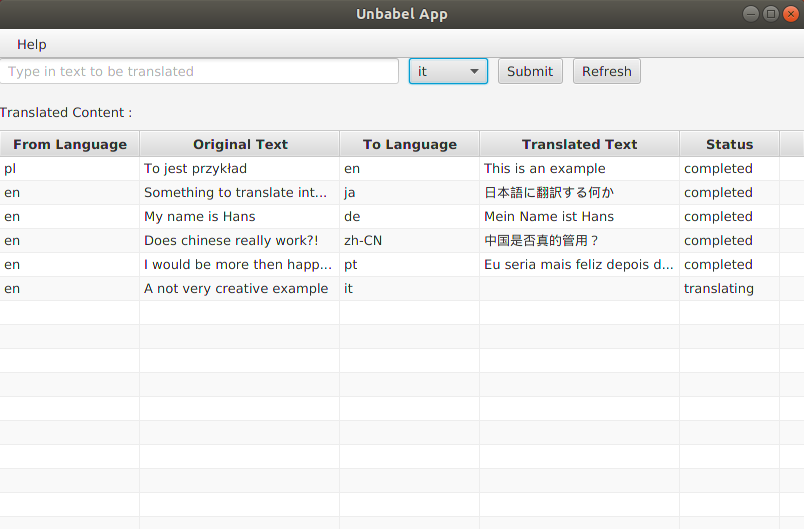
\includegraphics[scale=0.5]{appExample.png}
\caption{An example of the application user interface.}
\label{fig:app}
\end{figure}
The user interface consists of 
\begin{itemize}
\item A \texttt{TextField} where the user inputs the text to be translated.
\item A \texttt{ChoiceBox} with the available languages. 
\item Two \texttt{Button}s to submit the translation request and refresh the status of the request
\item A \texttt{TableView} to store all the user queries.
\item A \texttt{MenuBar} for future options such as \textit{save,file,help,etc.}
\end{itemize}

\subsection{Model}
The model takes care of all the user translation requests through the \texttt{HttpURLConnectionHandler} class. The class sends \texttt{POST} and \texttt{GET} requests using a \texttt{HttpsURLConnection} object from the \texttt{javax.net.ssl.HttpsURLConnection} package. When the user clicks on the \textit{Submit} \texttt{Button} a \texttt{GET} request is sent to the Unbabel API. All data sent and received to and from the Unbabel API is stored and transferred between objects through the \texttt{Translation} class. Then when using the \textit{Refresh} \texttt{Button} the \texttt{Model} according to the \textit{Status} of the query either sends a \texttt{GET} request to check whether the translation is completed or resends the request (\texttt{POST}) in case of errors or failures. This simple approach proves to be surprisingly error resistant which is necessary when working with web applications.

\subsection{Tests}
For the sole purpose of this application I have decided to write my own \texttt{JsonParser} class to parse all \texttt{JSON} objects.In the future this should be replaced with a more reliable tool such as \texttt{Gson}. But for my simple needs my implementation was more then enough. The \texttt{JsonParser} class was also a great opportunity to write \textit{Unit tests}. For this purpose I have used \texttt{JUnit5}. My tests can be found in the \texttt{JsonParserTest} class, which tests all the use cases in my application.

\section{Scalability and Future Improvements}
\begin{itemize}

\item The \texttt{Translation} class allows for easy adding of new features and translation parameters.
\item Possible target languges used in the \texttt{ChoiceBox} should be replaced for example with an \texttt{Enum} which would provide greater flexibilty in adding new languages and getting the code languages in different forms (e.g. for user and model purposes).
\item The \texttt{JsonParser} class should be replaced with a more reliable tool such as \texttt{Gson}. 
\item More test cases should be considered. Not only for \texttt{JSON} parsing but also fro \texttt{HTTP} connections and other features.
\end{itemize}
\end{document}